 \documentclass{article}

% Language setting
% Replace `english' with e.g. `spanish' to change the document language
 \usepackage[utf8]{inputenc}

% Set page size and margins
% Replace `letterpaper' with `a4paper' for UK/EU standard size

\documentclass{article}
\usepackage{pgfplots}
\pgfplotsset{width=10cm,compat=1.9}

% We will externalize the figures
\usepgfplotslibrary{external}
\tikzexternalize


\usepackage[letterpaper,top=2cm,bottom=2cm,left=3cm,right=3cm,marginparwidth=1.75cm]{geometry}

% Useful packages
\usepackage{amsmath}
\usepackage{float}
\usepackage{graphicx}
\usepackage[colorlinks=true, allcolors=blue]{hyperref}
\usepackage{listings}
\usepackage{xcolor}
\lstset { 
    language=C++,
    backgroundcolor=\color{black!5}, 
    basicstyle=\footnotesize,
    breaklines=true
}

\title{IT45 : Rapport de Développement\\
[0.3em] 
\Large
Problèmes d’affectation, de planification et de routage des
tournées des employés }

\author{Garbriel SCHWAB, Cyrille STROESSER}

\date{Printemps 2022}
\begin{document}
\maketitle

\vspace*{4cm}

\begin{figure}[h] 
    \center 
    
\includegraphics[scale=0.5]{utbm_forword-2.jpg} 
\end{figure}
\newpage
\tableofcontents

\newpage
\section{Introduction}

L'objectif de ce projet d'IT45 vise à résoudre un problème de recherche opérationnelle concret. Celui-ci à pour but d'affecter une liste de missions commandée à un SESSAD à ses employés de façon à optimiser plusieurs critères tout en respectant différentes contraintes. Les trois critères principaux d'optimisation son : 
\begin{enumerate}
  \item L’équité et l’égalité entre les employés en harmonisant la charge de travail et la distance parcourue.
  \item Les préf́erences des apprenants en minimisant le nombre des affectations dont la spécialité est insatisfaite.
  \item L’objectif du centre SESSAD en minimisant le nombre d’heures suppĺementaires et perdues et la distance totale parcourue.
\end{enumerate}
Pour résoudre ce problème, nous avons implémenté un algorithme génétique optimisé en casacade. Pour ce faire, il faut d'abord générer une population initiale avec des solutions valides et hétérogènes. Puis, il faut générer de nouvelles populations avec des croisements et des mutations pour en sélectionner les meilleurs individus selon le premier critère d'optimisation. Après un certain nombre d'itération, on sélectionne les meilleurs individus selon le deuxième critère d'optimisation et finalement on choisit le meilleur individu selon le derniers critère. Ensuite, il s'agit de trouver les meilleurs paramètres (taux de croisements, de mutations, méthode de séléction, population, itération,...) pour trouver la meilleure solution possible.
\newline

\newpage
\newpage

\section{Modélisation}
        \begin{figure}[h]
        \centering
        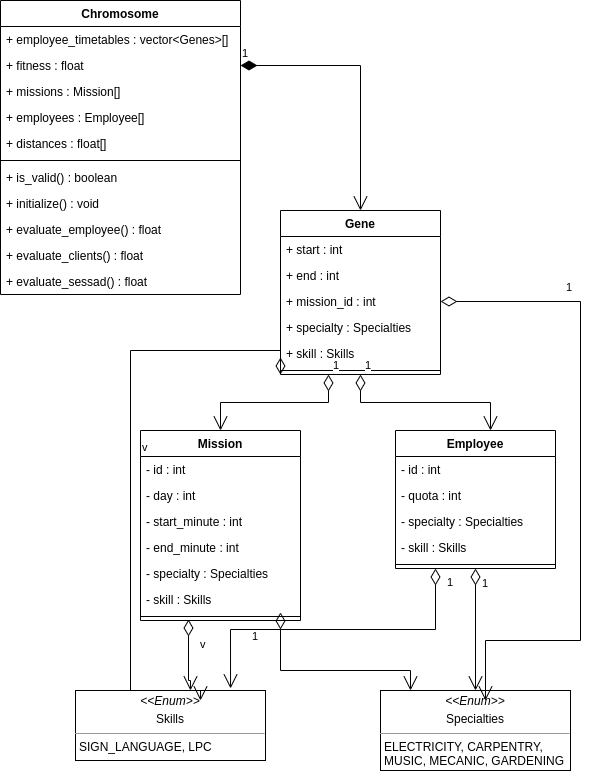
\includegraphics[width=0.7\textwidth]{class_diagram.png}
        \caption{\label{fig:class_diagram}Digramme de classe}
        \end{figure}
\newpage
\section{Implémentation}
    Nous avons choisi d'implémenter notre solution en C++ par souci de performance. En effet, ce langage permet une gestion de la mémoire bas niveau. Cela nous a permis d'optimiser au mieux la mémoire utilisée. En outre, nous maîtrisions déjà ce langage. 
    \subsection{Structure de données}
    Afin d'implémenter la modélisation détaillée ci-dessus, nous avons choisi différentes structures de données :
    \begin{itemize}
    \item \boldsymbol{Missions\ et\ Employés} : après avoir extrait les instances des fichiers \emph{csv}, les missions et intervenants (employees) sont stockées dans les structures suivantes : 
    \begin{lstlisting}
typedef struct
{
    int id;
    int day;
    int start_minute;
    int end_minute;
    Specialties specialty;
    Skills skill;
} Mission;
typedef struct
{
    int id;
    int quota;
    Specialties specialty;
    Skills skill;
} Mission;
    \end{lstlisting}
    \item \boldsymbol{Matrice\ des\ distances}: 
    Quant à la matrice des distances, bien que ce soit une matrice à deux dimensions, il est possible de la stocker dans un tableau à une dimension. Pour accéder à l'élément de la ligne i et de la colonne j, on utilise le code suivant :
    \begin{lstlisting}
// j = matrix size
distances[i*n_location + j];
    \end{lstlisting}
    Nous avons fait ce choix par souci d'optimisation, car parcourir un tableau à une dimension est nettement plus rapide pour un ordinateur que parcourir un tableau à deux dimensions.
    \item \boldsymbol{Gène}: 
    Un gène correspond à une affectation d'une mission sur un emploi du temps d'un employé. Il comprend toutes les informations nécessaires à l'optimisation de la solution (horaires, spécialité et compétence).
    \begin{lstlisting}
typedef struct
{
    int start;
    int end;
    int mission_id;
    Specialties specialty;
    Skills skill;
} Gene;
    \end{lstlisting}
    \item \boldsymbol{Chromosome} : les solutions, aussi appelées chromosomes, sont stockées dans une classe car leur manipulation par l'algorithme génétique rend l'utilisation de méthodes pertinente. Un chromosome est composé d'un objectif, d'un pointeur sur le tableau d'employés, d'un pointeur sur le tableau de missions et d'un pointeur sur la matrice des distances. Il est aussi composé d'un tableau de listes, $std::vector$, stockant les emplois du temps de tous les employés.
    \begin{lstlisting}
class Chromosome
{
public:
    float fitness;
    const Mission *missions;
    const Employee *employees;
    const float *distances;
    std::vector<Gene> *employee_timetables;
}
\end{lstlisting}
    De la même manière que la matrice des distances, $employee\_timetables$ est un tableau à deux dimensions, (jour de la semaine \textbf{x} nombre d'employés) ramené à une dimension. Pour accéder au jour $j$ de l'employé $k$, on utilise le code suivant :
\begin{lstlisting}
// N_WEEK_DAY = nombre de jours de le semaine
employee_timetables[k * N_WEEK_DAY + j];
\end{lstlisting}
    On accède alors à une liste de gène correspondants aux différents missions affectées à l'employées ce jour-ci. Cette liste est toujours triée dans l'ordre croissant pour former un emploi du temps.  
    \end{itemize}
    
    \subsection{Population initiale}
    Notre algorithme de génération de la solution initiale ne nécessite pas d'assouplissement de contrainte car il génére des solutions respectant toutes les contraintes strictement. Pour ce faire nous avons implémenter l'algorithme \textbf{first-fit}. Pour chaque mission, il suffit de l'affecter au premier jour du premier employé qui respecte toutes les contraintes. La solution va alors dépendre de l'ordre dans lequel est donné les missions ou de l'ordre dans lequel est donné les employés. Ainsi, pour pouvoir générer pleins de solutions initiales hétérogènes, il nous suffit de mélanger le tableau des missions et des employés avant de les passer dans l'algorithme de génération. Pour ce faire, on utilise la fonction suivante suivante :
\begin{lstlisting}
void initialize_population(Chromosome *population, const Mission missions_p[], const Employee employees_p[], const float distances_p[])
{
    population[0] = Chromosome(missions_p, employees_p, distances_p);
    population[0].initialize();

    for (int i = 1; i < population_size; ++i)
    {
        Mission missions[n_mission];
        Employee employees[n_employee];
        std::copy(missions_p, missions_p + n_mission, missions);
        std::copy(employees_p, employees_p + n_employee, employees);
        std::shuffle(missions, missions + n_mission, std::default_random_engine(i));
        std::shuffle(employees, employees + n_employee, std::default_random_engine(i));
        population[i] = Chromosome(missions, employees, distances_p);
        population[i].initialize();
    }
}
\end{lstlisting}
    L'objectif principal est d'avoir une population initiale composée de différentes solutions, diversifiées et de qualités. Il est important d'avoir un bon équilibre entre ces deux critères. Si nous avons une population trop diversifiée et très peu optimale, l'algorithme risque de ne pas être très efficace et de prendre trop de temps à converger. A l'inverse, si la population initiale est très optimale mais peu diversifiée, le risque est de tomber dans des optimums locaux
    \newline
    \newpage
    \subsection{Algorithme génétique}
        \subsubsection{Fitness}
        Nous avons repris les fonction d'évaluation proposées dans le sujet. Nous allons opter pour une résolution en cascade, c'est à dire que nous allons faire tourner notre algorithme avec la première fitness, puis filtrer les solutions obtenues avec les deux autres fonctions.
        Voici les fonctions d'évaluation que nous allons utiliser : 
        \begin{center}
        \begin{Large}
        \newline
        $f_{employees} = \frac{\zeta \cdot \sigma_{WH}(s)+ \gamma \cdot \sigma_{OH}(s) + \kappa \cdot \sigma_D(s)}{3}$
        \newline
        \bigskip
        $f_{clients} = \alpha \cdot penalties(s)$
        \newline
        \bigskip
        $f_{SESSAD} = \frac{\beta \cdot sumWOH(s) + \kappa \cdot moyD(s) + \kappa \cdot maxD(s) }{3} $
        \end{Large}
        \end{center}
        \newline 
        avec :
        \newline
        – $\sigma_{WH}(s)$ = écart type des heures non-travaillées des employés pour s
        \newline
        – $\sigma_{OH}(s)$ = écart type des heures supplémentaires des employés pour s
        \newline
        - $\sigma_{D}(s)$ = écart type des distances des employés pour s
        \newline
        - $penalties(s)$ = nombre d'affectation dont la spécialité est insatisfaite
        \newline
        - $\sigma_{WH}(s)$ = somme des heures non-travaillées et supplémentaires de tous les employés pour s
        \newline
        -  $moyD(s)$ = distance moyenne parcourue par les employés pour s
        \newline 
        - $maxD(s)$ = distance maximale parcourue par les employés pour s
        \newline
        - $ \alpha, \beta, \gamma, \zeta, \kapps$ sont des facteurs de corrélation.

        \subsubsection{Sélection}
        Pour sélectionner les meilleurs chromosomes destinés à être se reproduire entre eux, nous avons choisi d'utiliser une méthode de sélection proportionnelle, la sélection par roulette. Elle choisi les meilleurs chromosome ayant les meilleurs fitness. Ce choix nécessite d'avoir une population de départ très diversifiée pour ne pas rester bloqué dans des optimums locaux. Comme nous sommes dans le cas d'une minimisation d'objectif, la probabilité d'être séléctionner est donnée par la formule suivante : 
        \everymath{\displaystyle}
        %\begin{center}
        $\mathbb{P} = \frac{\frac{1}{F_p}}{\sum_{i}^{} \frac{1}{F_i}}$ ,  $F_p$ la fitness de l'individu
        \newline
        Nous l'avons implémenté  de la manière suivante :
\begin{lstlisting}
Chromosome *roulette_selection(Chromosome population[], std::default_random_engine &generator)
{
    float proba_sum = 0;
    float fitness_sum = 0;
    float proba_array[population_size] = {0};
    std::uniform_real_distribution<float> uniform_dist(0, 1);

    for (int i = 0; i < population_size; ++i){
        fitness_sum += 1 / population[i].evaluate_employees();
    }
    for (int i = 0; i < population_size; ++i){
        proba_array[i] = proba_sum + (1 / population[i].fitness) / fitness_sum;
        proba_sum += (1 / population[i].fitness) / fitness_sum;
    }

    size_t index = 0;
    float random = uniform_dist(generator);
    while (proba_array[index] < random)
        index++;

    return &population[index];
}
\end{lstlisting}
        \subsubsection{Croisement}
        Dans un premier temps, afin d'obtenir les meilleurs résultats et performances il faudra faire varier le taux de croisement, correspondant à la probabilité qu'un croisement ait lieu entre deux chromsomes au sein d'une même population. Ce dernier ce trouve dans l'intervalle $[0.2, 0.8]$.
        \newline
        \newline
        Nous avons testé plusieurs opérateurs de croisement mais nous en avons gardé seulement 2 :
        \begin{itemize}
        \item \boldsymbol{Day\ 1X} : cet opérateur sépare le cromosome en un point et l'enfant reçoit la première partie du premier parent et la deuxième partie du deuxième parent. Pour notre problème, la séparation en 2 se fait au milieu de la semaine. C'est à dire que lorsqu'on résonne en terme d'emploi du temps, l'enfant va recevoir toutes les affectations de missions du Lundi et du Mardi du parent 1 par exemple, et toutes les affectations de missions du Mercredi, Jeudi et Vendredi du parent 2. 
        \item \boldsymbol{Days\ NX} : de la même manière que le \emph{Day 1X}, cet opérateur procède à un échange de journées entre deux chromosomes, mais au lieu de scinder le chromosomem en deux, on le scinde en autant de parties qu'il y a de jours de travail. Ainsi, un enfant peu recevoir toutes les affectations de mission du Lundi du parent 1, toutes les affectations de missions du Mardi du parent 2, toutes les affectations des missions du Mercredi du parent 1, etc ...
        \end{itemize}
        Nous avons garder uniquement ces deux opérateurs de croisement, car ceux-ci nous assuraient d'obtenir une solution valide après chaque croisement. Le problème à résoudre étant assez complexe et les contraintes assez dures à respecter totalement, il n'y avait pas beaucoup d'opérateurs de croisement permettant d'obtenir des solutions valides à chaque fois. Voici notre l'implémentation de l'opérateur de croisement \boldsymbol{Day\ 1X} :
        \begin{lstlisting}
void crossover_1X(Chromosome *parent1, Chromosome *parent2, Chromosome *child1, Chromosome *child2)
{
    for (int i = 0; i < n_employee; ++i)
    {
        child1->employee_timetables[i * N_WEEK_DAY + MONDAY] = parent1->employee_timetables[i * N_WEEK_DAY + MONDAY];
        child1->employee_timetables[i * N_WEEK_DAY + TUESDAY] = parent1->employee_timetables[i * N_WEEK_DAY + TUESDAY];
        child1->employee_timetables[i * N_WEEK_DAY + WEDNESDAY] = parent1->employee_timetables[i * N_WEEK_DAY + WEDNESDAY];
        child1->employee_timetables[i * N_WEEK_DAY + THURSDAY] = parent2->employee_timetables[i * N_WEEK_DAY + THURSDAY];
        child1->employee_timetables[i * N_WEEK_DAY + FRIDAY] = parent2->employee_timetables[i * N_WEEK_DAY + FRIDAY];

        child2->employee_timetables[i * N_WEEK_DAY + MONDAY] = parent2->employee_timetables[i * N_WEEK_DAY + MONDAY];
        child2->employee_timetables[i * N_WEEK_DAY + TUESDAY] = parent2->employee_timetables[i * N_WEEK_DAY + TUESDAY];
        child2->employee_timetables[i * N_WEEK_DAY + WEDNESDAY] = parent2->employee_timetables[i * N_WEEK_DAY + WEDNESDAY];
        child2->employee_timetables[i * N_WEEK_DAY + THURSDAY] = parent1->employee_timetables[i * N_WEEK_DAY + THURSDAY];
        child2->employee_timetables[i * N_WEEK_DAY + FRIDAY] = parent1->employee_timetables[i * N_WEEK_DAY + FRIDAY];
    }
}
\end{lstlisting}
        \newpage
        \subsubsection{Mutation}
        Pour ce qui est des mutations, elles s'effectuent sur une partie de la population. Une mutation apparaît sur certains individus avec une propabilité définie par le taux de mutation. Pour conserver au maximum la validité de notre population, les opérateurs de mutation permuttent des missions d'employés ayant la même compétence.
        \begin{itemize}  
        \item \boldsymbol{Full\ swap} : cet opérateur de mutation permutte une journée entière de deux employés.
        \item \boldsymbol{Rand\ swap} : cet opérateur agit aussi sur deux employés et permutte toutes les missions commençant par une heure choisie aléatoirement.
        \end{itemize}
        Voici l'implémentation du \boldsymbol{Full\ swap}:
        \begin{lstlisting}
        void mutate_full_swap(Chromosome *chromosome, const Employee employees[], std::default_random_engine &generator)
{
    int day;
    int employee_index2;
    int employee_index1;
    std::uniform_int_distribution<int> uniform_dist_emp(0, n_employee - 1);
    std::uniform_int_distribution<int> uniform_dist_day(0, N_WEEK_DAY - 1);

    day = uniform_dist_day(generator);
    employee_index2 = uniform_dist_emp(generator);
    employee_index1 = uniform_dist_emp(generator);
    while (employees[employee_index1].skill != employees[employee_index2].skill || employee_index1 == employee_index2)
        employee_index2 = uniform_dist_emp(generator);

    Chromosome temp_chromosome = *chromosome;

    temp_chromosome.employee_timetables[employee_index2 * N_WEEK_DAY + day] = chromosome->employee_timetables[employee_index1 * N_WEEK_DAY + day];
    temp_chromosome.employee_timetables[employee_index1 * N_WEEK_DAY + day] = chromosome->employee_timetables[employee_index2 * N_WEEK_DAY + day];

    if(temp_chromosome.is_valid()){
        chromosome->employee_timetables[employee_index1*N_WEEK_DAY + day] = temp_chromosome.employee_timetables[employee_index1 * N_WEEK_DAY + day];
        chromosome->employee_timetables[employee_index2*N_WEEK_DAY + day] = temp_chromosome.employee_timetables[employee_index2 * N_WEEK_DAY + day];
    } 
}
        \end{lstlisting}
    
    \newpage
    \subsection{Optimisations diverses}
    Par soucis de performances, nous avons effectué un certain nombre d'optimisations dans notre implémentation. En effet, le C++ nous offre une grande marge de manoeuvre quant à la gestion des ressources que nous avons exploité dans les optimisations suivantes : 
    \begin{itemize} 
        \item $i++$ est un opérateur à proscrire pour simplement incrémenter $i$ car il stocke la valeur de $i$ avant son incrémentation et la retourne. Pour éviter ce gachis de ressource nous utilisons l'opérateur $++i$ pour incrémenter nos variables.
        \item Nous utilisons au maximum le passage de variables par adresse ou par référence quand celles-ci sont en lecture-seul. Cela évite d'utiliser de la mémoire pour des éléments destinés uniquement à être lus.
        \Nous avons utilisé des tableaux à une dimension pour représenter des tableaux à deux dimensions afin d'avoir une mémoire continu, cela rend l'accès aux données plus rapide.
        \item Afin de ne pas laisser des itérations tourner inutilement, nous utilisons les opérateurs $break;$ et $continue;$ au maximum pour stoper les boucles lorsque les itérations suivantes ne sont plus nécessaires.
        \item Nous utilisons peu de variables globales, et nous passons tous nos tableaux en paramètres car l'accès à une variable globale demande plus de ressources que l'accès aux paramètres de la fonction.
        \item Nous avons utilisé les flags de compilation \emph{-O3} et \emph{-flto} pour que le compilateur réalise des optimisations de notre code au moment de la compilation.
    
    \end{itemize}
    
\newpage
\section{Benchmark}
Afin de trouver les meilleurs paramètres pour générer la meilleure solution possible nous avons implémenté une fonction $benchmark$. Cette fonction résoud plusieurs fois le problème avec des paramètres différents et stocke le résultat de chaque résolution dans un fichier benchmark.txt. Cela permet de constater l'influence des paramètres sur les résultats. Pour réaliser les benchmarks sur chaque instance nous avons choisis les paramètres suivants :
\begin{itemize}
    \item itération = 50\ 000
    \item population = 50
    \item taux de mutation  = \{0.2,0.3,0.4,0.5\}
    \item taux de croisement = \{0.2,0.4,0.6,0.8\}
\end{itemize}


\begin{figure}[H]\centering
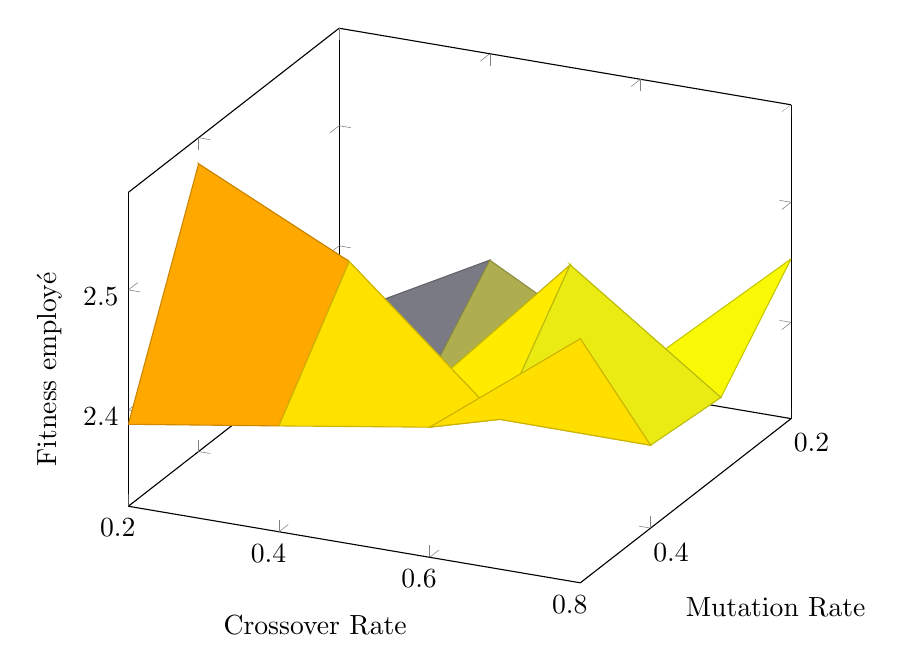
\begin{tikzpicture}
\begin{axis}[
y dir=reverse,
zlabel = Fitness employé,
ylabel = Mutation Rate,
xlabel = Crossover Rate,
]
\addplot3[
    surf,
] 
coordinates {

(0.2,0.2,2.34166) (0.2,0.3,2.41297) (0.2,0.4,2.55937) (0.2,0.5,2.38812)

(0.4,0.2,2.40929) (0.4,0.3,2.34171) (0.4,0.4,2.49926) (0.4,0.5,2.40802)

(0.6,0.2,2.34166) (0.6,0.3,2.47213) (0.6,0.4,2.38915) (0.6,0.5,2.42821)

(0.8,0.2,2.4529)(0.8,0.3,2.38302) (0.8,0.4,2.38885) (0.8,0.5,2.52309)

};
\end{axis}
\end{tikzpicture}
\caption{Instance 96}
\end{figure}


\begin{figure}[H]\centering
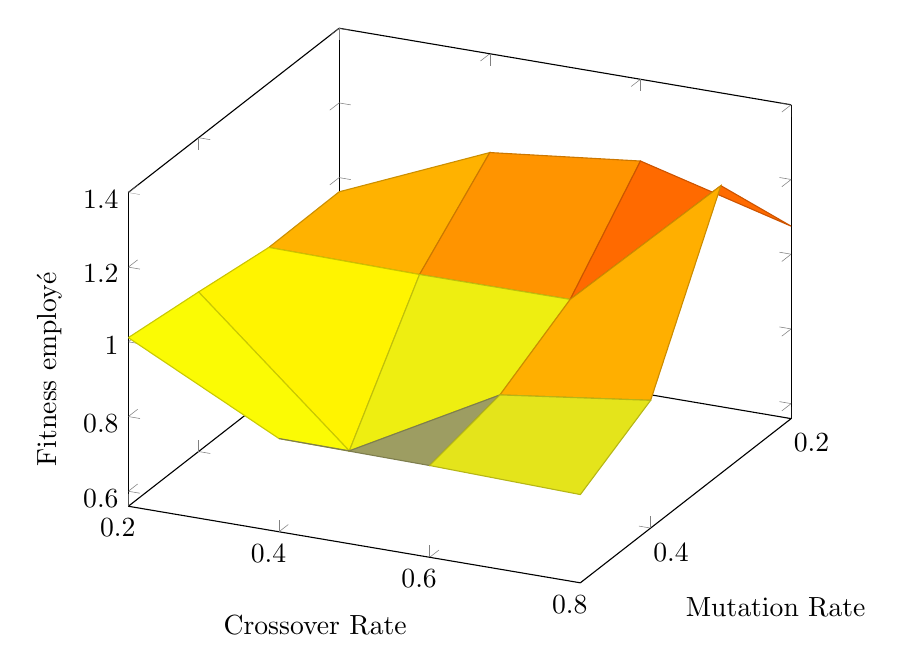
\begin{tikzpicture}
\begin{axis}[
y dir=reverse,
zlabel = Fitness employé,
ylabel = Mutation Rate,
xlabel = Crossover Rate,
]
\addplot3[
    surf,
] 
coordinates {

(0.2,0.2,0.962008) (0.2,0.3,0.959653) (0.2,0.4,0.987027) (0.2,0.5,1.0112)

(0.4,0.2,1.13546) (0.4,0.3,0.955527) (0.4,0.4,0.629868) (0.4,0.5,0.809357)

(0.6,0.2,1.18108) (0.6,0.3,0.957178) (0.6,0.4,0.847986) (0.6,0.5,0.805501)

(0.8,0.2,1.075) (0.8,0.3,1.32995) (0.8,0.4,0.901823) (0.8,0.5,0.796119)

};
\end{axis}
\end{tikzpicture}
\caption{Instance 96}
\end{figure}

\begin{figure}[h]\centering

\caption{figure caption}
\label{fig:...}
\end{figure}

\begin{figure}[H]\centering
%% 50 000 itérations population 50
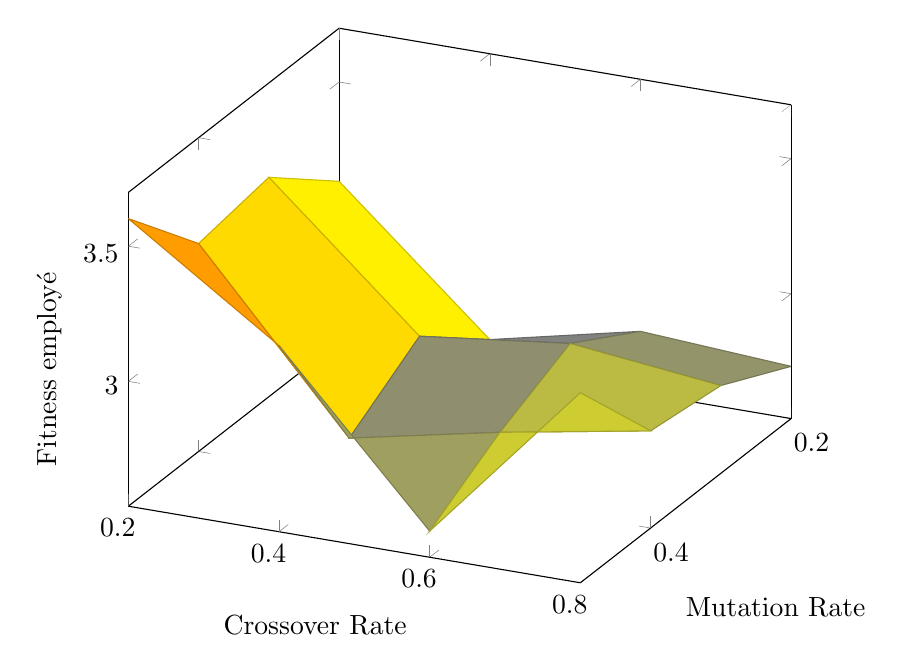
\begin{tikzpicture}
\begin{axis}[
y dir=reverse,
zlabel = Fitness employé,
ylabel = Mutation Rate,
xlabel = Crossover Rate,
]
\addplot3[
    surf,
] 
coordinates {
(0.2,0.2,3.1324) (0.2,0.3,3.34978) (0.2,0.4,3.30729) (0.2,0.5,3.60219)

(0.4,0.2,2.64135) (0.4,0.3,2.85614) (0.4,0.4,2.68154) (0.4,0.5,3.2266)

(0.6,0.2,2.7662) (0.6,0.3,2.92388) (0.6,0.4,2.7977) (0.6,0.5,2.63467)

(0.8,0.2,2.73108) (0.8,0.3,2.86281) (0.8,0.4,2.89761) (0.8,0.5,3.24124)

};
\end{axis}
\end{tikzpicture}
\caption{Instance 100}
\end{figure}

\newline
Afin de mieux comprednre ces résultats nous les avons affiché sous forme de graphique (voir figure ci-dessus). En abscisse on retrouve le taux de mutation, en ordonnée, le taux de croisement et en côte la première fitness. Sur la figure 2, on constate l'importance des mutations et des croisements car plus le taux de ces deux paramètres est élevé, plus la fitness est basse. La figure 3 nous confirme l'importance des croisements car plus le taux de croisement est élevé plus la fitness est basse. Cependant ce n'est pas une science exacte car la figure 1 est inexploitable.


\end{document}